
\documentclass[tikz]{standalone}
\usepackage{graphicx}
\usepackage{lmodern}
\usepackage{amsmath, amssymb, amsfonts}
\usetikzlibrary{calc}
\newcommand{\R}{\mathcal{R}}

\begin{document}

%abstain alpha = 1/2
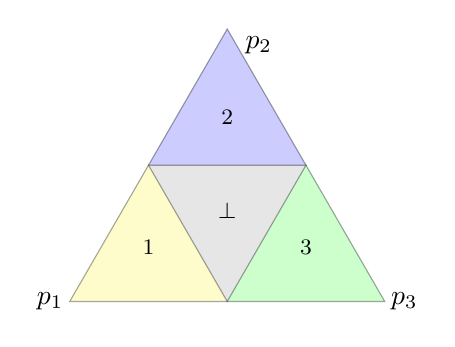
\begin{tikzpicture}
\draw[opacity = 0.2] (2,0) -- (-2,0) -- (0,3.46) -- cycle;
%label outcomes
\node at (-9/4, 0) {$p_1$};
\node at (2/5, 3.25) {$p_2$};
\node at (9/4, 0) {$p_3$};
%level sets
\draw[fill = blue, fill opacity = 0.1, opacity = 0.2] (-1, 1.73) -- (1, 1.73) -- (0, 3.46) -- cycle; 
\node at (0, 1.73*1.35) {\footnotesize$2$};
\draw[fill = green, fill opacity = 0.1, opacity = 0.2] (2,0) -- (1, 1.73) -- (0,0) -- cycle;
\node at (1, 1.73*0.4) {\footnotesize$3$};
\draw[fill = yellow, fill opacity = 0.1, opacity = 0.2] (-2,0) -- (-1, 1.73) -- (0,0) -- cycle;
\node at (-1, 1.73*0.4) {\footnotesize$1$};
\draw[fill = gray, fill opacity = 0.1, opacity = 0.2] (1,1.73) -- (-1, 1.73) -- (0,0) -- cycle;
\node at (0, 1.1533) {\footnotesize$\bot$};


\end{tikzpicture}

%ranking
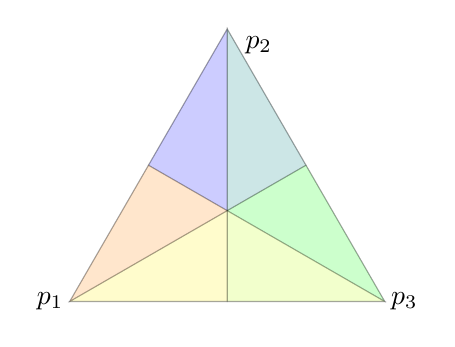
\begin{tikzpicture}
\draw[opacity = 0.2] (2,0) -- (-2,0) -- (0,3.46) -- cycle;
%label outcomes
\node at (-9/4, 0) {$p_1$};
\node at (2/5, 3.25) {$p_2$};
\node at (9/4, 0) {$p_3$};
%level sets
\draw[fill = blue, fill opacity = 0.1, opacity = 0.2] (-1, 1.73) -- (0, 1.1533) -- (0, 3.46) -- cycle; 
%\node[rotate=90] at (-1/4, 1.73*1.25) {\footnotesize$2 \prec 1 \prec 3$};
\draw[fill = teal, fill opacity = 0.1, opacity = 0.2] (1, 1.73) -- (0, 1.1533) -- (0, 3.46) -- cycle; 
%\node[rotate=90] at (1/4, 1.73*1.25) {\footnotesize$2 \prec 3 \prec 1$};
\draw[fill = green, fill opacity = 0.1, opacity = 0.2] (2,0) -- (1, 1.73) -- (0,1.1533) -- cycle;
%\node[rotate=-30] at (1, 1.73*.45) {\footnotesize$3 \prec 2 \prec 1$};
\draw[fill = lime, fill opacity = 0.8, opacity = 0.2] (2,0) -- (0, 0) -- (0,1.1533) -- cycle;
%\node[rotate=0] at (0.7, 0.2) {\footnotesize$3 \prec 1 \prec 2$};
\draw[fill = yellow, fill opacity = 0.1, opacity = 0.2] (-2,0) -- (0, 1.1533) -- (0,0) -- cycle;
%\node[rotate=0] at (-0.7, 0.2) {\footnotesize$1 \prec 3 \prec 2$};
\draw[fill = orange, fill opacity = 0.1, opacity = 0.2] (-2,0) -- (0, 1.1533) -- (-1,1.73) -- cycle;
%\node[rotate=30] at (-1, 1.73*.45) {\footnotesize$1 \prec 2 \prec 3$};


\end{tikzpicture}


%top- 2
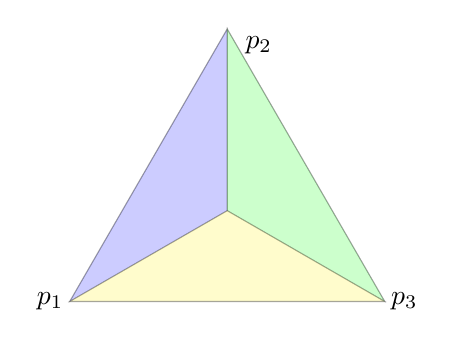
\begin{tikzpicture}
\draw[opacity = 0.2] (2,0) -- (-2,0) -- (0,3.46) -- cycle;
%label outcomes
\node at (-9/4, 0) {$p_1$};
\node at (2/5, 3.25) {$p_2$};
\node at (9/4, 0) {$p_3$};
%level sets
\draw[fill = blue, fill opacity = 0.1, opacity = 0.2] (-2, 0) -- (0, 1.1533) -- (0, 3.46) -- cycle; 
%\node at (-0.5, 1.73) {\footnotesize$(1,2)$};
\draw[fill = green, fill opacity = 0.1, opacity = 0.2] (2,0) -- (0,3.46) -- (0,1.1533) -- cycle;
%\node at (0.5, 1.73) {\footnotesize$(2,3)$};
\draw[fill = yellow, fill opacity = 0.1, opacity = 0.2] (-2,0) -- (0, 1.1533) -- (2,0) -- cycle;
%\node at (0, 1.73*0.3) {\footnotesize$(1,3)$};



\end{tikzpicture}





\end{document}
%%% Local Variables:
%%% mode: latex
%%% TeX-master: t
%%% End:
